\section{Planificación}
\subsection[Diagrama de Gantt]{Diagrama de Gantt}
En esta sección se muestra una diagrama de Gantt con la planificación del proyecto dividido en diferentes tareas. La figura que contiene el diagrama \ref{fig:gantt} se encuentra al final de esta sección. Las tareas en las que se ha dividido el proyecto son las siguientes:
\begin{itemize}
	\item \textbf{Investigación sobre el problema:} en esta tarea se realizó un estudio del problema que se resuelve en este Trabajo de Fin de Grado.
	\item \textbf{Investigación sobre herramientas para el desarrollo:} en esta tarea se realizó un estudio sobre las herramientas disponibles para resolver el problema.
	\item \textbf{Análisis de requisitos:} en esta tarea se realizó un análisis de los requisitos de la aplicación a desarrollar.
	\item \textbf{Diseño:} en esta tarea se explicó los diferentes aspectos del diseño de la aplicación.
	\item \textbf{Implementación:} en esta tarea se explicó los aspectos más importantes desarrollado en la aplicación.
	\item \textbf{Evaluación y pruebas:} en esta tarea se realizaron pruebas sobre diferentes casos de uso de la aplicación por parte de un usuario.
\end{itemize}

\subsection[Herramientas utilizadas para la planificación]{Herramientas utilizadas para la planificación}
\subsubsection{Trello}
Trello \cite{trello} es una herramienta muy utilizada en el ámbito empresarial. Trello consiste en tableros en los cuales se incluyen tareas. Dichas tareas pueden moverse de un tablero a otro y pueden asignarse si es necesario a personas concretas.\newline

Para este Trabajo de Fin de Grado, se ha creado un tablero al que se le ha llamado \enquote*{TFG} y se han utilizado tres tablas: Lista de tareas, En proceso y Finalizado. En la tabla \enquote*{Lista de tareas} se encuentran todas las tareas programadas que aún no se han empezado; en la tabla \enquote*{En proceso} se encuentran todas las tareas que se están desarrollando y en el tabla \enquote*{Finalizado} se encuentran todas las tareas que se han finalizado.
\subsubsection{GitHub}
GitHub \cite{github} es un servicio que permite almacenar proyectos utilizando el sistema de control de versiones Git. GitHub es gratuito para todas las personas que quieran crear repositorios visibles para todo el mundo; si se desea crear repositorio privados hay que contratar un plan de pago.\newline

Para este Trabajo de Fin de Grado, se ha utilizado GitHub para crear un repositorio que contenga el proyecto e ir subiendo nuevas versiones de este cuando se han completados tareas dentro del proyecto.\newline
\newpage
\begin{figure}[H]
	\centering
	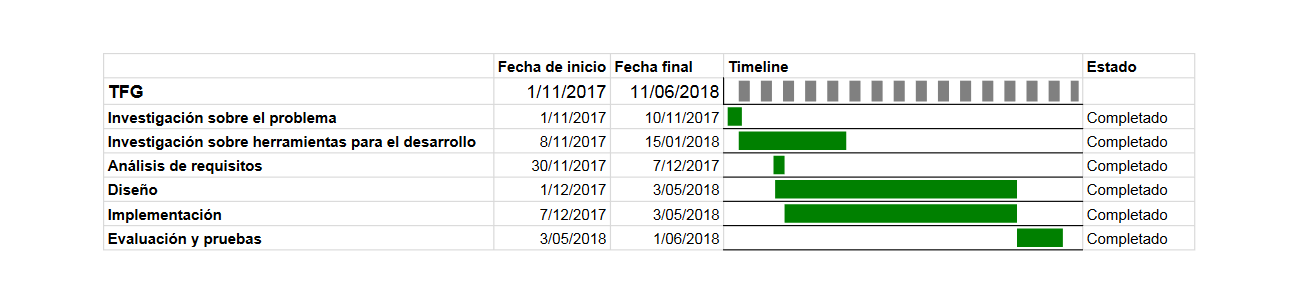
\includegraphics[scale=0.55,angle=90]{imagenes/Gantt.png}
	\caption{Planificación del proyecto.}
	\label{fig:gantt}
\end{figure}
